\colorlet{ind}{black}
\colorlet{dep}{gray!50!white}
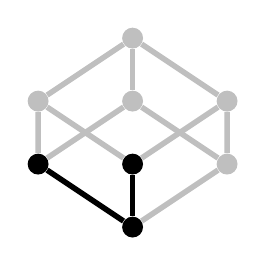
\begin{tikzpicture}[scale=0.8, every node/.style={scale=0.8}]
  \draw (0, 0)    node[circle, fill, color=ind] (o) {};
  \draw (-1.5, 1) node[circle, fill, color=ind] (a) {};
  \draw (0, 1)    node[circle, fill, color=ind] (b) {};
  \draw (1.5, 1)  node[circle, fill, color=dep] (c) {};
  \draw (-1.5, 2) node[circle, fill, color=dep] (ab) {};
  \draw (0, 2)    node[circle, fill, color=dep] (ac) {};
  \draw (1.5, 2)  node[circle, fill, color=dep] (bc) {};
  \draw (0, 3)    node[circle, fill, color=dep] (abc) {};
  \draw[line width=2pt, color=dep] (abc) -- (ab);
  \draw[line width=2pt, color=dep] (abc) -- (ac);
  \draw[line width=2pt, color=dep] (abc) -- (bc);
  \draw[line width=2pt, color=dep] (ac) -- (a);
  \draw[line width=2pt, color=dep] (ac) -- (c);
  \draw[line width=2pt, color=dep] (ab) -- (a);
  \draw[line width=2pt, color=dep] (ab) -- (b);
  \draw[line width=2pt, color=dep] (bc) -- (b);
  \draw[line width=2pt, color=dep] (bc) -- (c);
  \draw[line width=2pt, color=ind] (a) -- (o);
  \draw[line width=2pt, color=ind] (b) -- (o);
  \draw[line width=2pt, color=dep] (c) -- (o);
\end{tikzpicture}